\chapter{Searches For Natural SUSY With B-tag Templates.}
\label{chap:templatemethod}


Within this chapter a complimentary technique is discussed as a means to predict the distribution of three and four reconstructed b-quark jets in an event. The recent discovery of the Higgs boson has made third-generation ``Natural \ac{SUSY}'' models attractive, given that light top and bottom squarks are a candidate to stabilise divergent loop corrections to the Higgs boson mass.

Using the $\alphat$ search as a base, a simple templated fit is employed to estimate the \ac{SM} background in higher b-tag multiplicities (3-4) from a region of a low number of reconstructed b-jets (0-2). As a proof- of-concept, the procedure after being shown to close in simulation, is applied to the SM enriched \mupjets control sample of the \alphat all-hadronic search detailed in Chapter \ref{chap:SUSYsearches}. . To highlight the relative insensitivity of the choice of the b-tagging algorithm working points in the effectiveness of the procedure, results are presented using the \ac{CSV} tagger (introduced in Section (\ref{subsec:cmsobjects-btagging})) for the ``Loose'', ``Medium'' and ``Tight'' working points.


\section{Concept}
\label{sec:templateconcept}

The dominant \ac{SM} backgrounds most \ac{SUSY} searches are typically \ttbar + jets, W + jets and \zinv + jets. These process are characterised by typically having zero or two underlying b-quarks per event. The first step in this approach is to categorise two templates to be fitted to the low $n_{b}^{reco}$ multiplicity in terms of these underlying b-quark event topologies :

\begin{itemize}
\item[Z0 -] W + jets, \zinv + jets, DY + jets 
\item[Z2 -] \ttbar, single top
\end{itemize}

where Z0 and Z2 represent processes which have an underlying b-quark content of zero or two respectively. 

Both these templates can be generated through the application of the relevant event selection and taking the underlying $n_{b}^{reco}$ distribution directly from simulation. However as discussed within Section (\ref{subsec:backgroundestimation}), there are large uncertainties for high $n_{b}^{reco}$ multiplicities due to limited MC statistics. This is particularly prominent for the Z0 templates, where the number of reconstructed b-tags is driven primarily by the light-quark mis-tagging rate.  Therefore to improve the statistical precision of the predictions the formula method, introduced in Section (\ref{subsec:formulamethod}) is used. 

The generation of these templates is then dependant upon the jet-flavour content and b-tagging rate within the phase space of interest, with the tagging probabilities of a jet being a function of the jet \pt, the pseudo-rapidity $\rvert\eta\lvert$, and the jet-flavour. This can be observed in Figure \ref{fig:templatetaggingefficiencies}, where the b-tagging / c-quark mis-tagging / light mis-tagging efficiency for the three working points of the \ac{CSV} tagger is shown as a function of jet \pt. 

\begin{figure}[ht]
\centering
\begin{minipage}[b]{0.48 \linewidth}
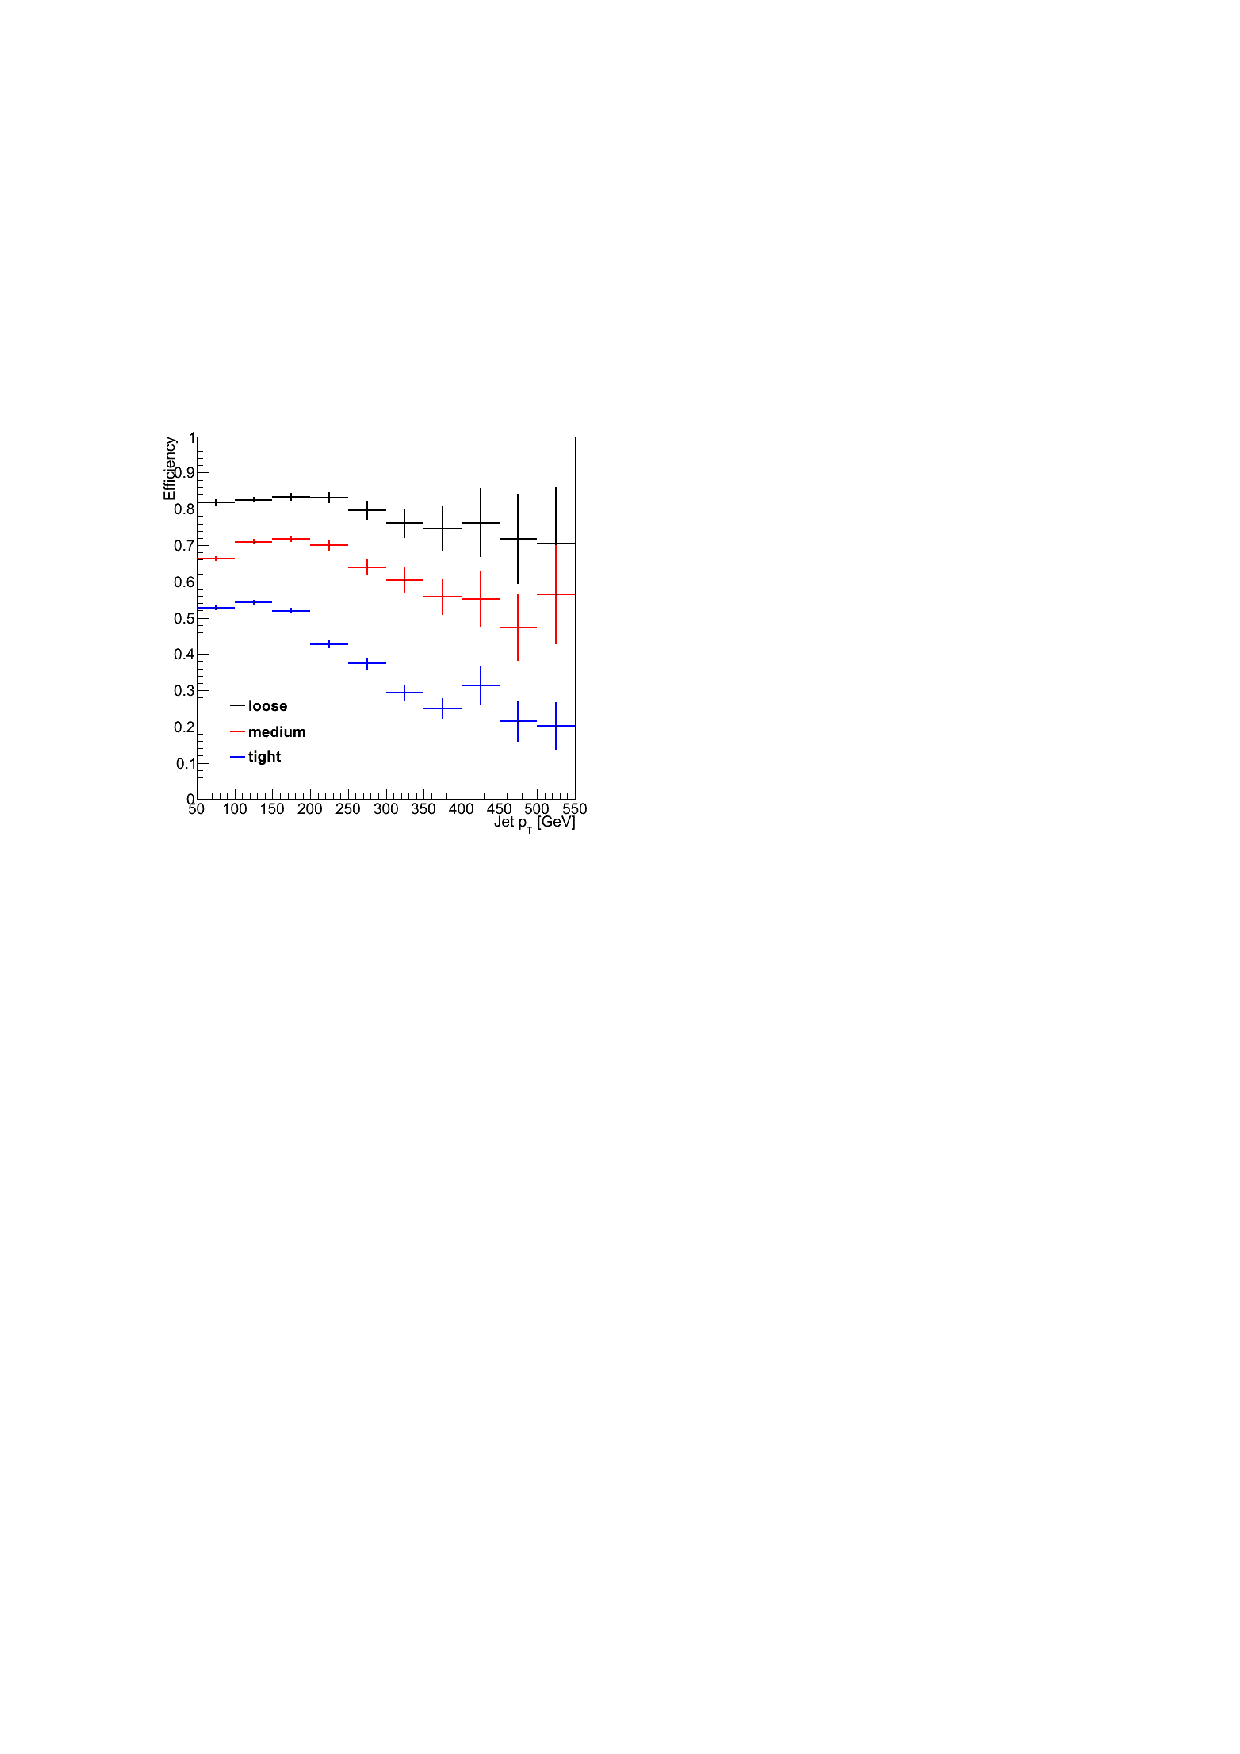
\includegraphics[width = 1.0\linewidth]{plots/template_btagrate.pdf}
\centering (a)  
\end{minipage}
\quad
\begin{minipage}[b]{0.48\linewidth}
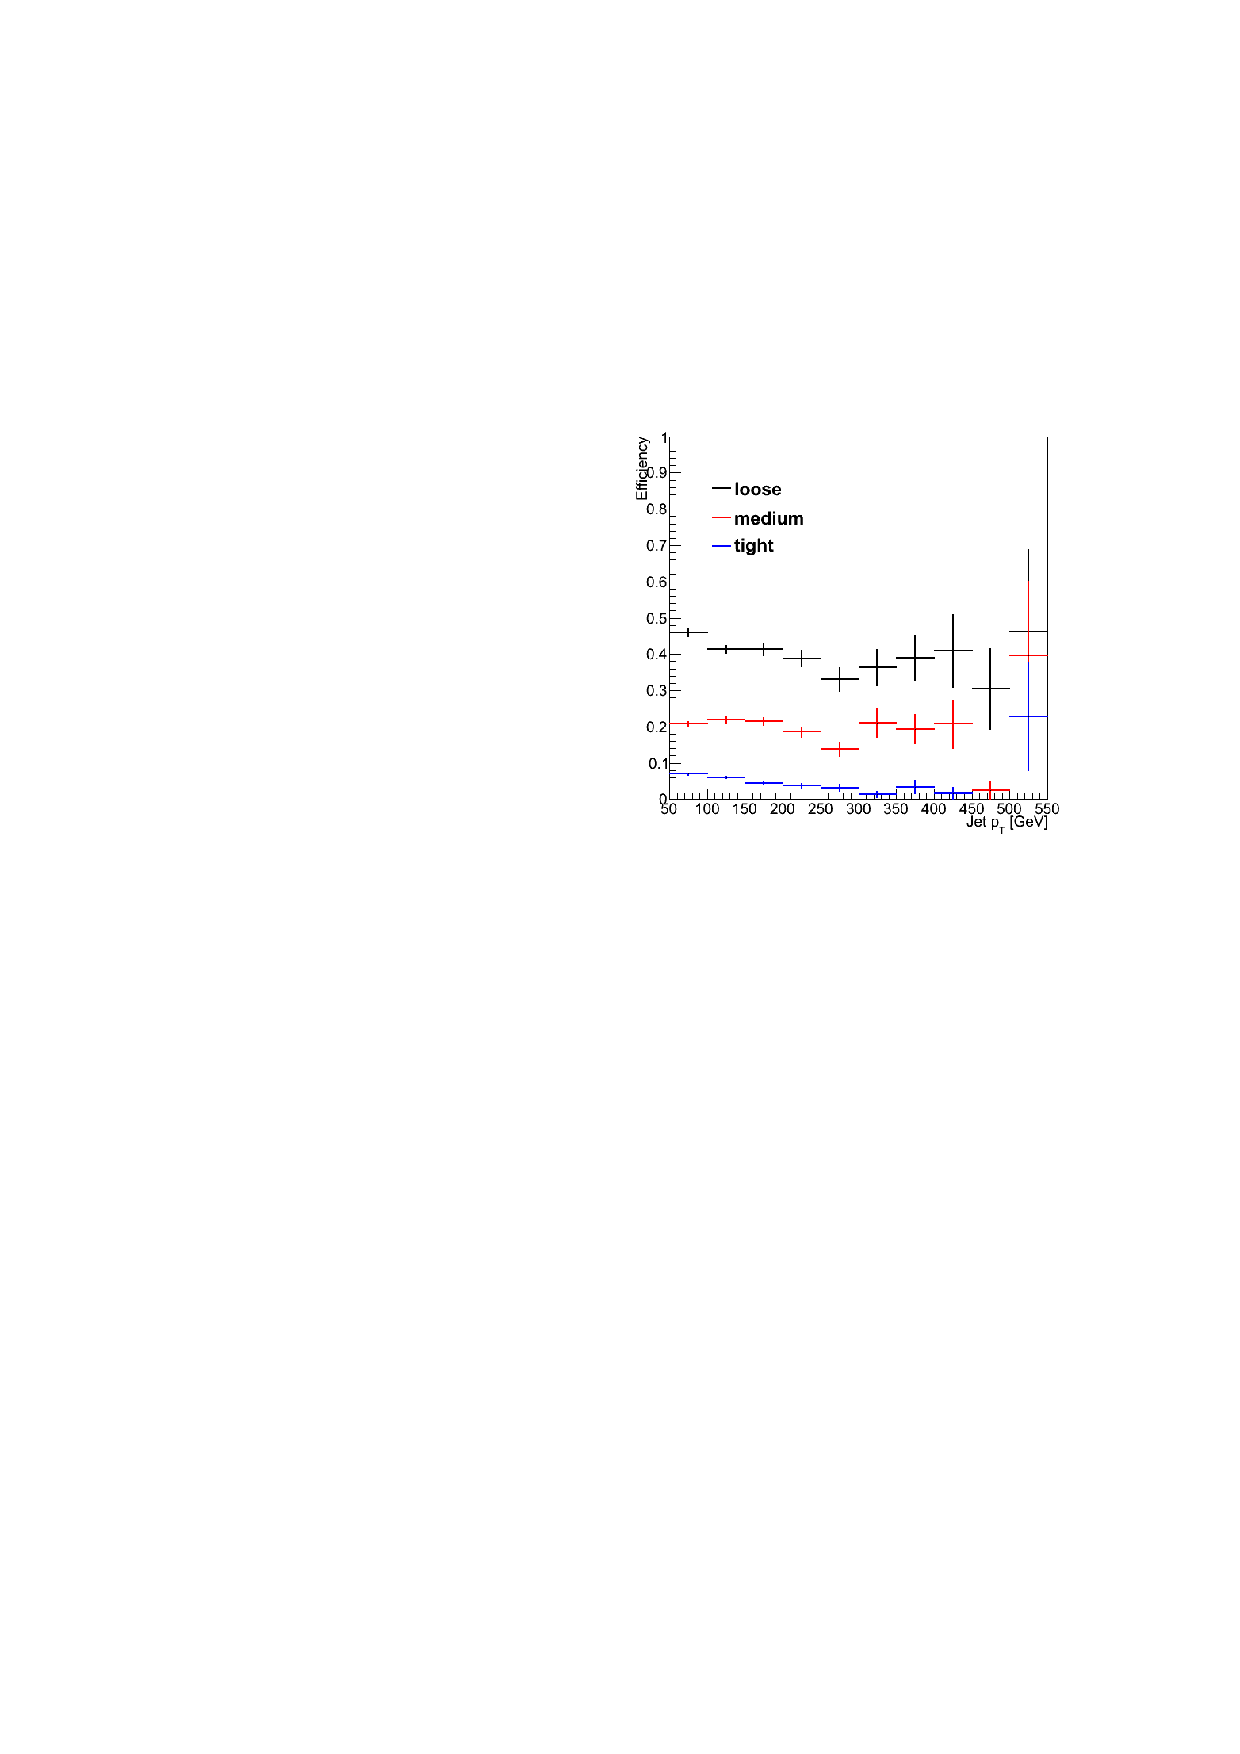
\includegraphics[width = 1.0\linewidth]{plots/template_ctagrate.pdf}
\centering (b) 
\end{minipage}
\quad
\begin{minipage}[b]{0.48\linewidth}
\centering
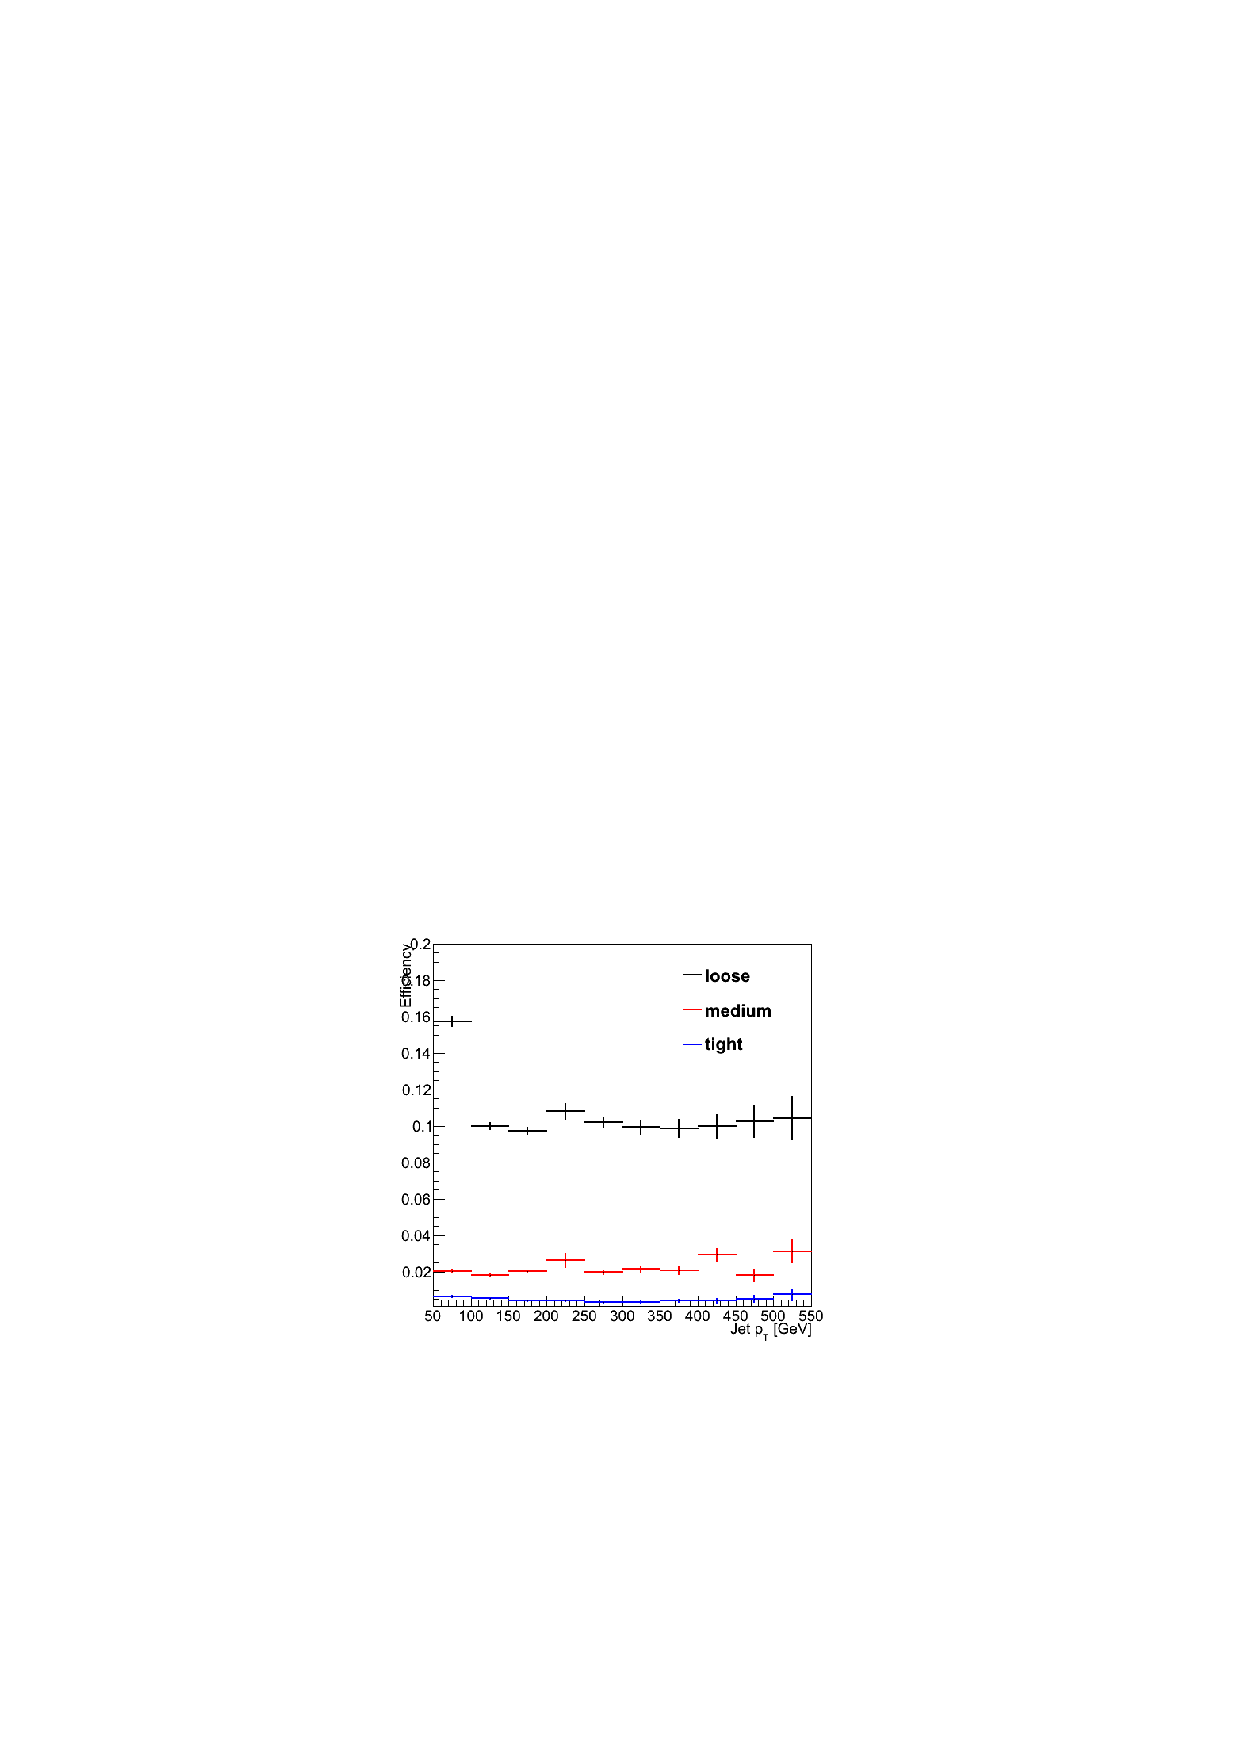
\includegraphics[width = 1.0\linewidth]{plots/template_mistagrate.pdf}
\centering (c) 
\end{minipage}
\caption[The b-tagging (a), c-quark mis-tagging (b), and light-quark mis-tagging rate (c$)$ as measured in simulation after the \alphat analysis, \mupjets control sample selection in the region \theht $>$ 375.]{The b-tagging (a), c-quark mis-tagging (b), and light-quark mis-tagging rate (c$)$ as measured in simulation after the \alphat analysis, \mupjets control sample selection in the region \theht $>$ 375.}
\label{fig:templatetaggingefficiencies}
\end{figure}

Before the templates are generated, the relevant jet \pt and \eta corrections are applied to correct simulation to data, as specified in Section (\ref{subsec:formulamethodsf}), to then determine the average tagging rates per analysis bin.   

These two templates are then fit to data in the low $n_{b}^{reco}$ region (0-2). The fit result is used, along with the knowledge of the template shapes, to extrapolate an estimate to the high $n_{b}^{reco}$ signal region (3,4), which is then compared to what is observed in data.

This method can, in principle, be applied to any analysis where the signal hypothesis has a larger underlying b-quark spectra than the \ac{SM} backgrounds, as it solely relies on fitting to the shape of the $n_{b}^{reco}$ distribution.

\section{ Application to the \alphat Search}
\label{sec:templateapplication}

As detailed in the previous chapter, the \alphat analysis is a search for \ac{SUSY} particles in all-hadronic final states, utilising the kinematic variable \alphat to suppress QCD to a negligible level. \ac{SM} enriched control samples are used to estimate the background within an all-hadronic signal region. 

The selection for the \mupjets control samples defined in Section (\ref{subsec:controlsampledefinition}) is used to demonstrate the template fitting procedure both conceptually in simulation, and also when applied in data. This is chosen, as such a selection is dominated by events stemming from the \ac{SM} processes with little or no signal contamination from potential new physics.. Neither are contributions from rate \ac{SM} processes with a higher underlying b-quark content (e.g. $t\bar{t}b\bar{b}$) expected. For these reasons, there is a degree of confidence that the procedure should close when applied to this phase space.

The analysis presented here is binning in source jet multiplicity bins, of 3,4 and $\geq$ 5 reconstructed jets per event (di-jet events are not included as there is no contribution to the high $n_{b}^{reco}$ region (3,4)) , in order to reduce the kinematic jet \pt dependence. Furthermore the analysis is split into three \theht regions, 

\begin{itemize}
\item 275-325 \GeV
\item 325-375 \GeV
\item $>$ 375 \GeV
\end{itemize}

contrary to the eight used within the \alphat analysis. Templates for both underlying b-quark content hypotheses are then generated for the nine defined analysis bins.

\subsection{Proof of principle in simulation}
\label{subsec:templateclosuretest}

In order to demonstrate that the template procedure produces accurate predictions within simulation, the simulation samples in the analysis are firstly split into two to allow for statistically independent fits to be performed. 

By combing the relevant ingredients necessary to employ the formula method, $n_{b}^{reco}$ templates for Z = 0 and Z= 2 are generated individually for each $n_{jet}$ and \theht bin using one half of each simulation sample. A fit of these two templates is then performed in the low $n_{b}^{reco}$ (0-2) region, back to the sum of the other halves of each simulation sample in order to check that the relevant information can be recovered in the $n_{b}^{reco}$ signal region (3-4).

The fits are performed independently within each of the defined analysis bins to reduce the dependence of the shapes of these distributions on simulation. The half of the simulation sample for which the templates are fitted too, are taken directly from simulation, extending this procedure to also be a validation of the formula method to accurately estimate the $n_{b}^{reco}$ distribution. Additionally as this test is performed in simulation, the relevant corrections of the b-tagging rates between data and simulation are \emph{not} applied.  

Within Figure \ref{fig:template_closure_njet5}, the results of this fitting procedure is shown for each \ac{CSV} working point. Results are presented for the $n_{jet} \geq 5$ category, using the \mupjets control sample selection in the inclusive \theht$>$ 375 \GeV analysis bin. The grey bands represent the statistical uncertainty on the template shapes. Additional fits are shown for other $n_{jet}$ category within Appendix \ref{app:templatemc}. 

Furthermore the extrapolated fit predictions within the high $n_{b}^{reco}$ signal region, are summarised for all \theht bins and working points in Table \ref{tab:template_mctable}. 

 \begin{table}[h!]
\begin{center}
\footnotesize
\begin{tabular*}{0.95\textwidth}{@{\extracolsep{\fill}}lccc}
\cline{1-4}
\multicolumn{1}{c}{\theht} & 275-325 & 325-375 & $>$375 \\

\multicolumn{4}{c}{Loose working point} \\
\hline\hline
Simulation $n_{b} = 3$ & $344.0 \pm 6.8$ & $158.8 \pm 4.5$ & $324.9 \pm 6.5$ \\ 
Template $n_{b} = 3$ & $347.5 \pm 11.6$ & $162.6 \pm 4.7$ & $322.9 \pm 6.9$ \\ 
Simulation $n_{b} = 4$ & $29.8 \pm 1.9$ & $11.1 \pm 1.1$ & $40.2 \pm 2.4$ \\ 
Template $n_{b} = 4$ & $32.6 \pm 2.0$ & $13.0 \pm 1.0$ & $37.0 \pm 1.8$ \\ 
\hline
\multicolumn{4}{c}{Medium working point} \\
\hline\hline
Simulation $n_{b} = 3$ & $58.2 \pm 2.87$ & $33.3 \pm 2.1$ & $72.1 \pm 3.1$ \\ 
Template $n_{b} = 3$ & $60.1 \pm 1.9$ & $32.1 \pm 1.5$ & $70.8 \pm 2.3$ \\ 
Simulation $n_{b} = 4$ & $1.0 \pm 0.4$ & $0.3 \pm 0.2$ & $1.5 \pm 0.4$ \\ 
Template $n_{b} = 4$ & $1.2 \pm 0.1$ & $0.4 \pm 0.1$ & $2.2 \pm 0.2$ \\ 
\hline
\multicolumn{4}{c}{Tight working point} \\
\hline\hline
Simulation $n_{b} = 3$ & $58.2 \pm 2.87$ & $33.3 \pm 2.1$ & $72.1 \pm 3.1$ \\ 
Template $n_{b} = 3$ & $60.1 \pm 1.9$ & $32.1 \pm 1.5$ & $70.8 \pm 2.3$ \\ 
Simulation $n_{b} = 4$ & $1.0 \pm 0.4$ & $0.3 \pm 0.2$ & $1.5 \pm 0.4$ \\ 
Template $n_{b} = 4$ & $1.2 \pm 0.1$ & $0.4 \pm 0.1$ & $2.2 \pm 0.2$ \\ 
\end{tabular*}
\end{center}
\caption[Summary of the fit predictions in the $n_{b}^{reco}$ signal region for $n_{jet} =3, =4, \geq 5$. The fit region is $n_{b}^{reco}$ = 0, 1, 2 and simulation yields are normalised to an integrated luminosity of 10 fb$^{-1}$. ]{Summary of the fit predictions in the $n_{b}^{reco}$ signal region for $n_{jet} = 3, =4, \geq 5$. The fit region is $n_{b}^{reco}$ = 0, 1, 2 and simulation yields are normalised to an integrated luminosity of 10 fb$^{-1}$.. The uncertainties quoted on the template yields are purely statistical.}\label{tab:template_mctable}
\end{table}


The pull distributions for all the fits performed are compatible with a mean of zero and standard distributions, see Appendix \ref{app:templatepulldistributions}.

The good overall agreement summarised in the table validates both the formula method used to generate the templates as well as the fitting method itself. The application of this method to the same selection in data is used to demonstrate necessary control over the efficiency and mis-tagging rates.

\begin{figure}[ht]
\centering
\begin{minipage}[b]{0.55 \linewidth}
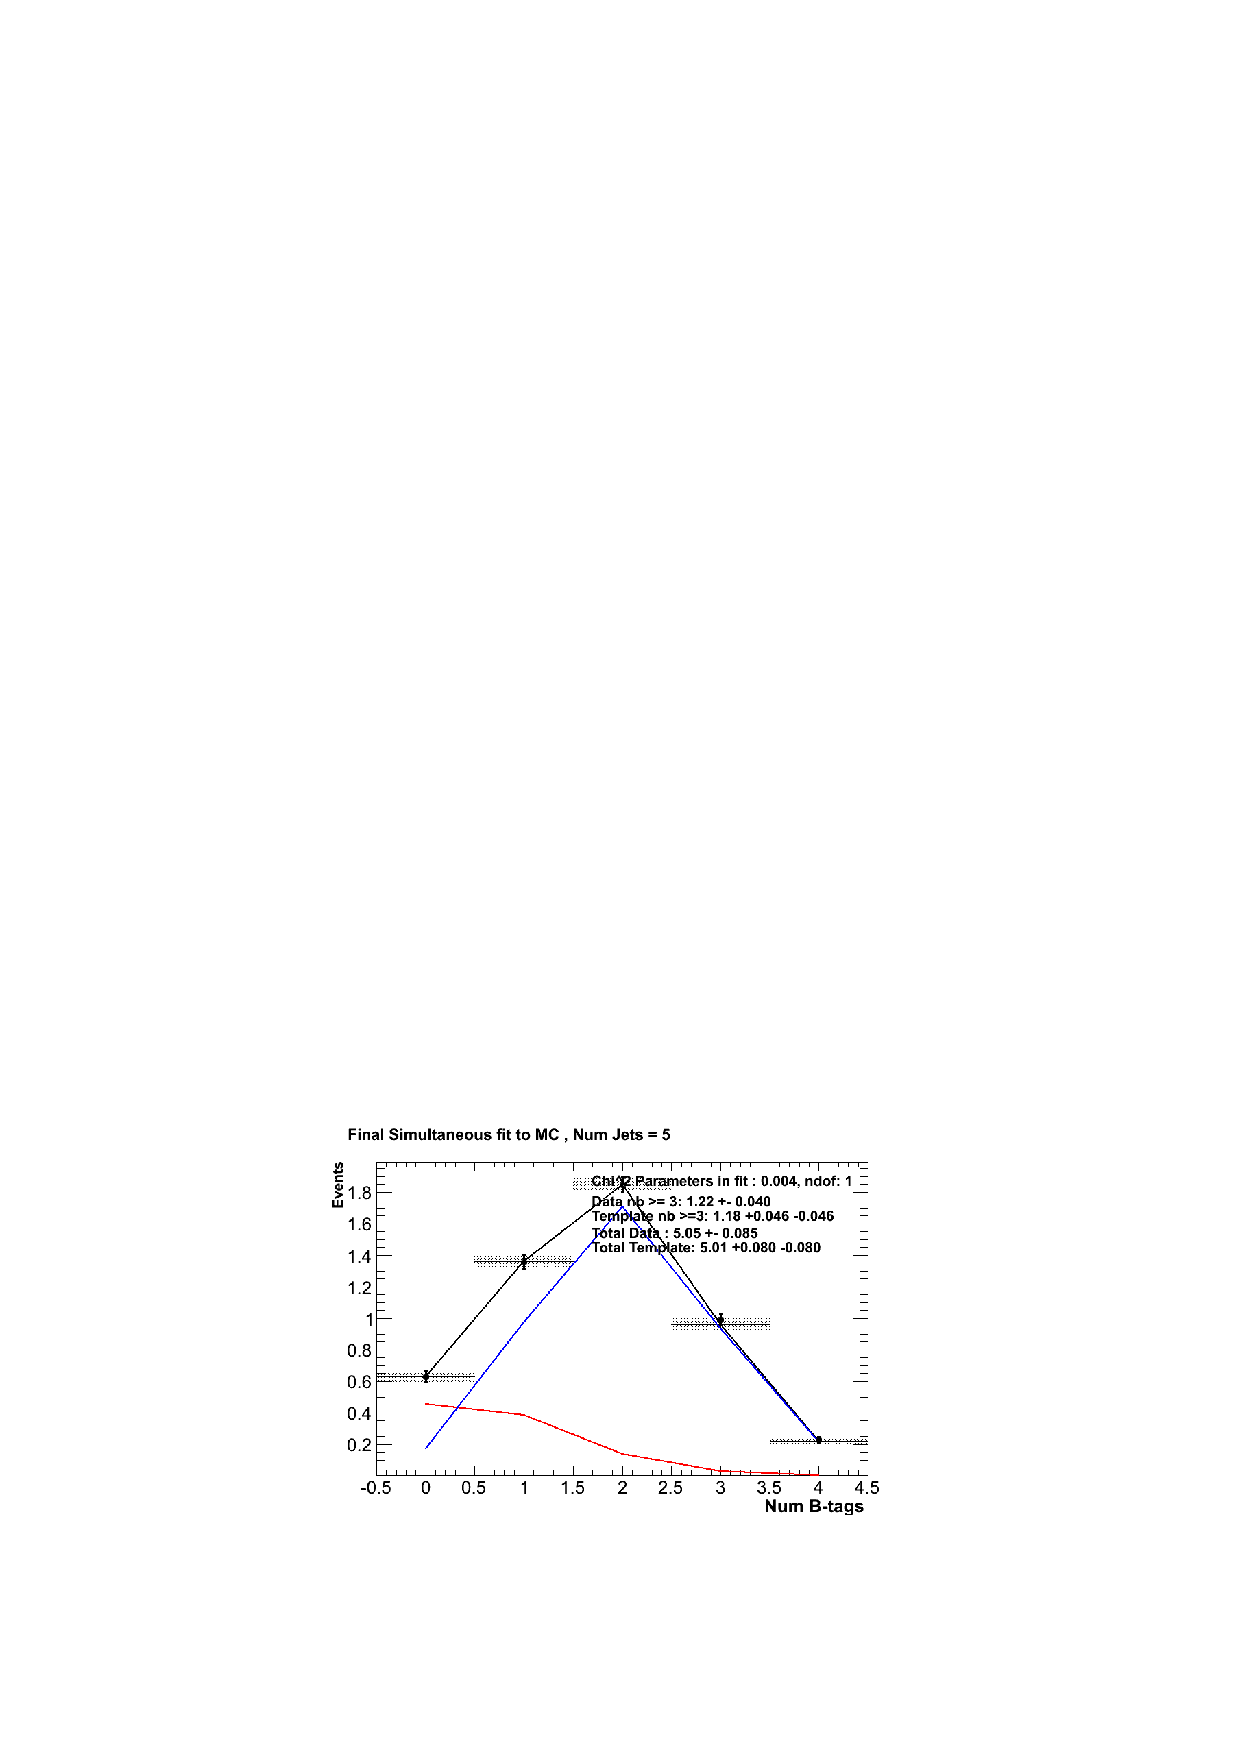
\includegraphics[width = 1.0\linewidth]{plots/template_mc_loose_njet5.pdf}
\centering (a) Loose working point : $n_{jet} \geq$  5 
\end{minipage}
\quad
\begin{minipage}[b]{0.55\linewidth}
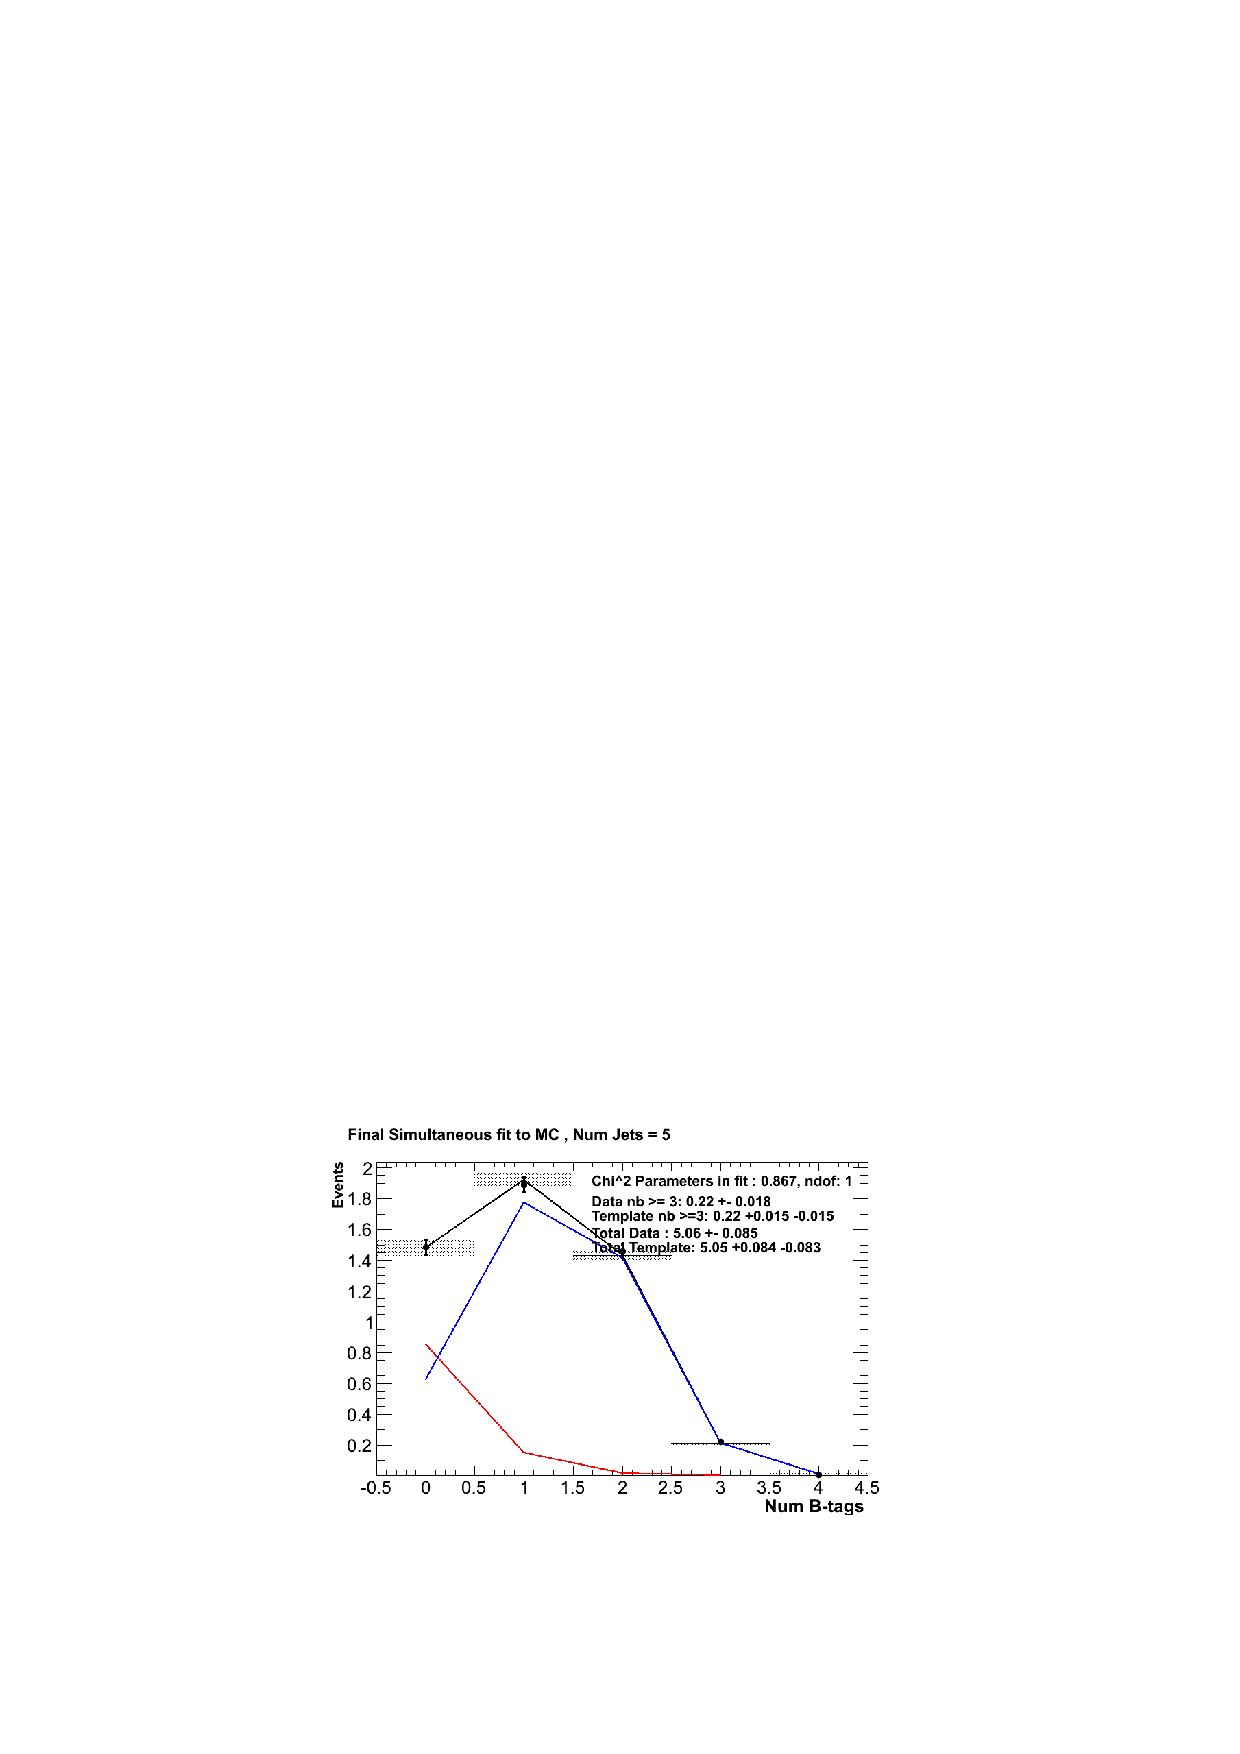
\includegraphics[width = 1.0\linewidth]{plots/template_mc_medium_njet5.pdf}
\centering (b) Medium working point : $n_{jet} \geq$ = 5 
\end{minipage}
\quad
\begin{minipage}[b]{0.55\linewidth}
\centering
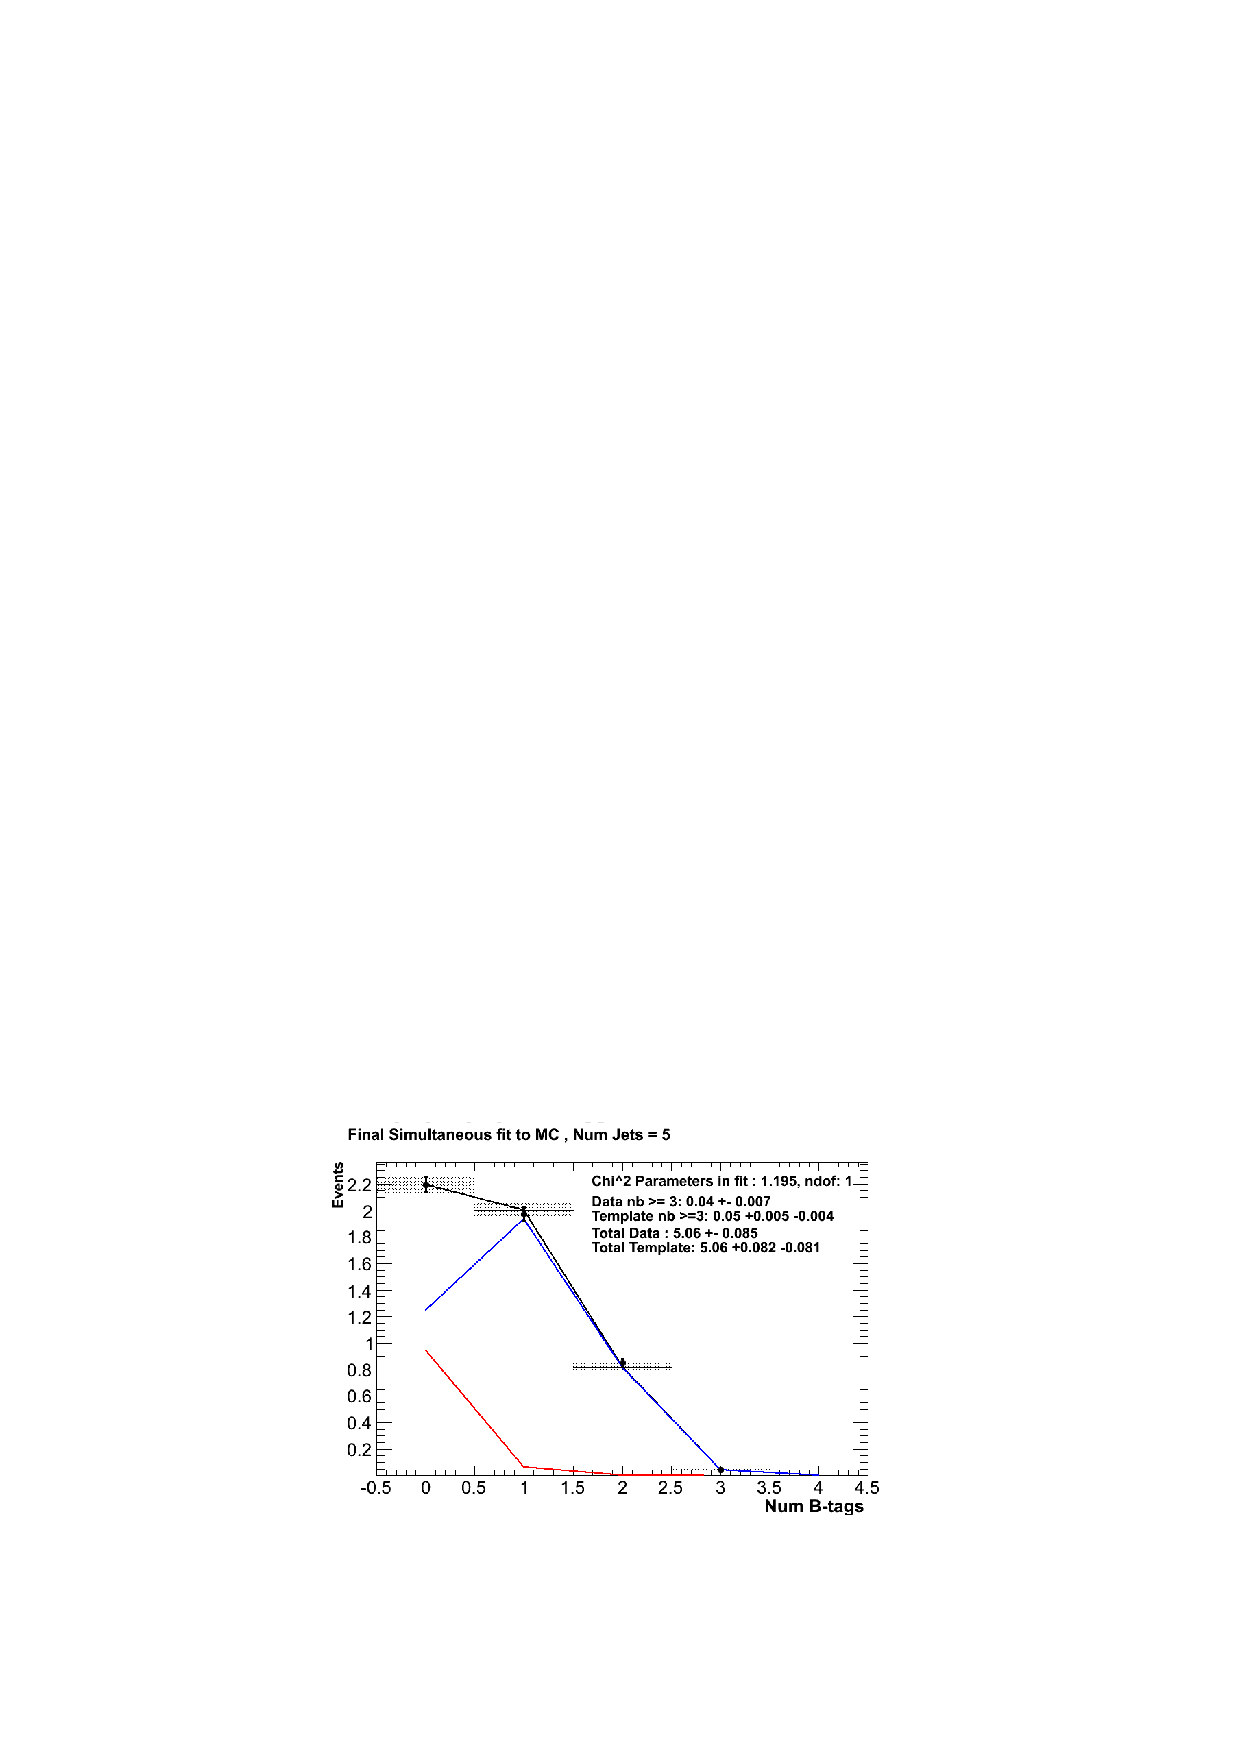
\includegraphics[width = 1.0\linewidth]{plots/template_mc_high_njet5.pdf}
\centering (c) Tight working point : $n_{jet} \geq$ 5 
\end{minipage}
\caption[The results of fitting the Z = 0 and Z = 2 templates to the $n_{b}^{reco}$ = 0, 1, 2 bins taken directly from simulation in the region \theht $>$ 375 \GeV, for the $n_{jet} \geq 5$ category.]{The results of fitting the Z = 0 and Z = 2 templates to the $n_{b}^{reco}$ = 0, 1, 2 bins taken directly from simulation in the region \theht $>$ 375 \GeV, for the $n_{jet} \geq 5$ category. The red template represents Z = 0, while the blue template represents Z = 2. Grey bands represent the statistical uncertainty of the fit. The $\chi^{2}$ parameter displayed represents the goodness of fit to the low$ n_{b}^{reco}$ (0-2) control region.}
\label{fig:template_closure_njet5}
\end{figure}

\FloatBarrier
\subsection{Results in a data control sample}
\label{subsec:templatedataresults}

The method above is now applied to the 2012 8 \TeV dataset in the \mupjets control sample, to establish the validity of this method in data. The relevant data to simulation scale factors are applied to get corrected values of the efficiency and mis-tagging rates measured in data \cite{btag8tev} \cite{btagscalefactor}. 

Figure \ref{fig:template_data_med_njet5} show the  the results of the templates derived from simulation to each of the three defined \theht bins, in the $n_{jet} \geq 5$ category for the medium working point \ac{CSV} tagger (the same working point used within the \alphat analysis).  Grey bands represent the statistical uncertainty of the fit combined in quadrature with the systematic uncertainties of varying the data to simulation scale factors up and down by their measured systematic uncertainties.  Additional fit results for the other working points are found in Appendix \ref{app:templatedata}  

\begin{figure}[ht]
\centering
\begin{minipage}[b]{0.55 \linewidth}
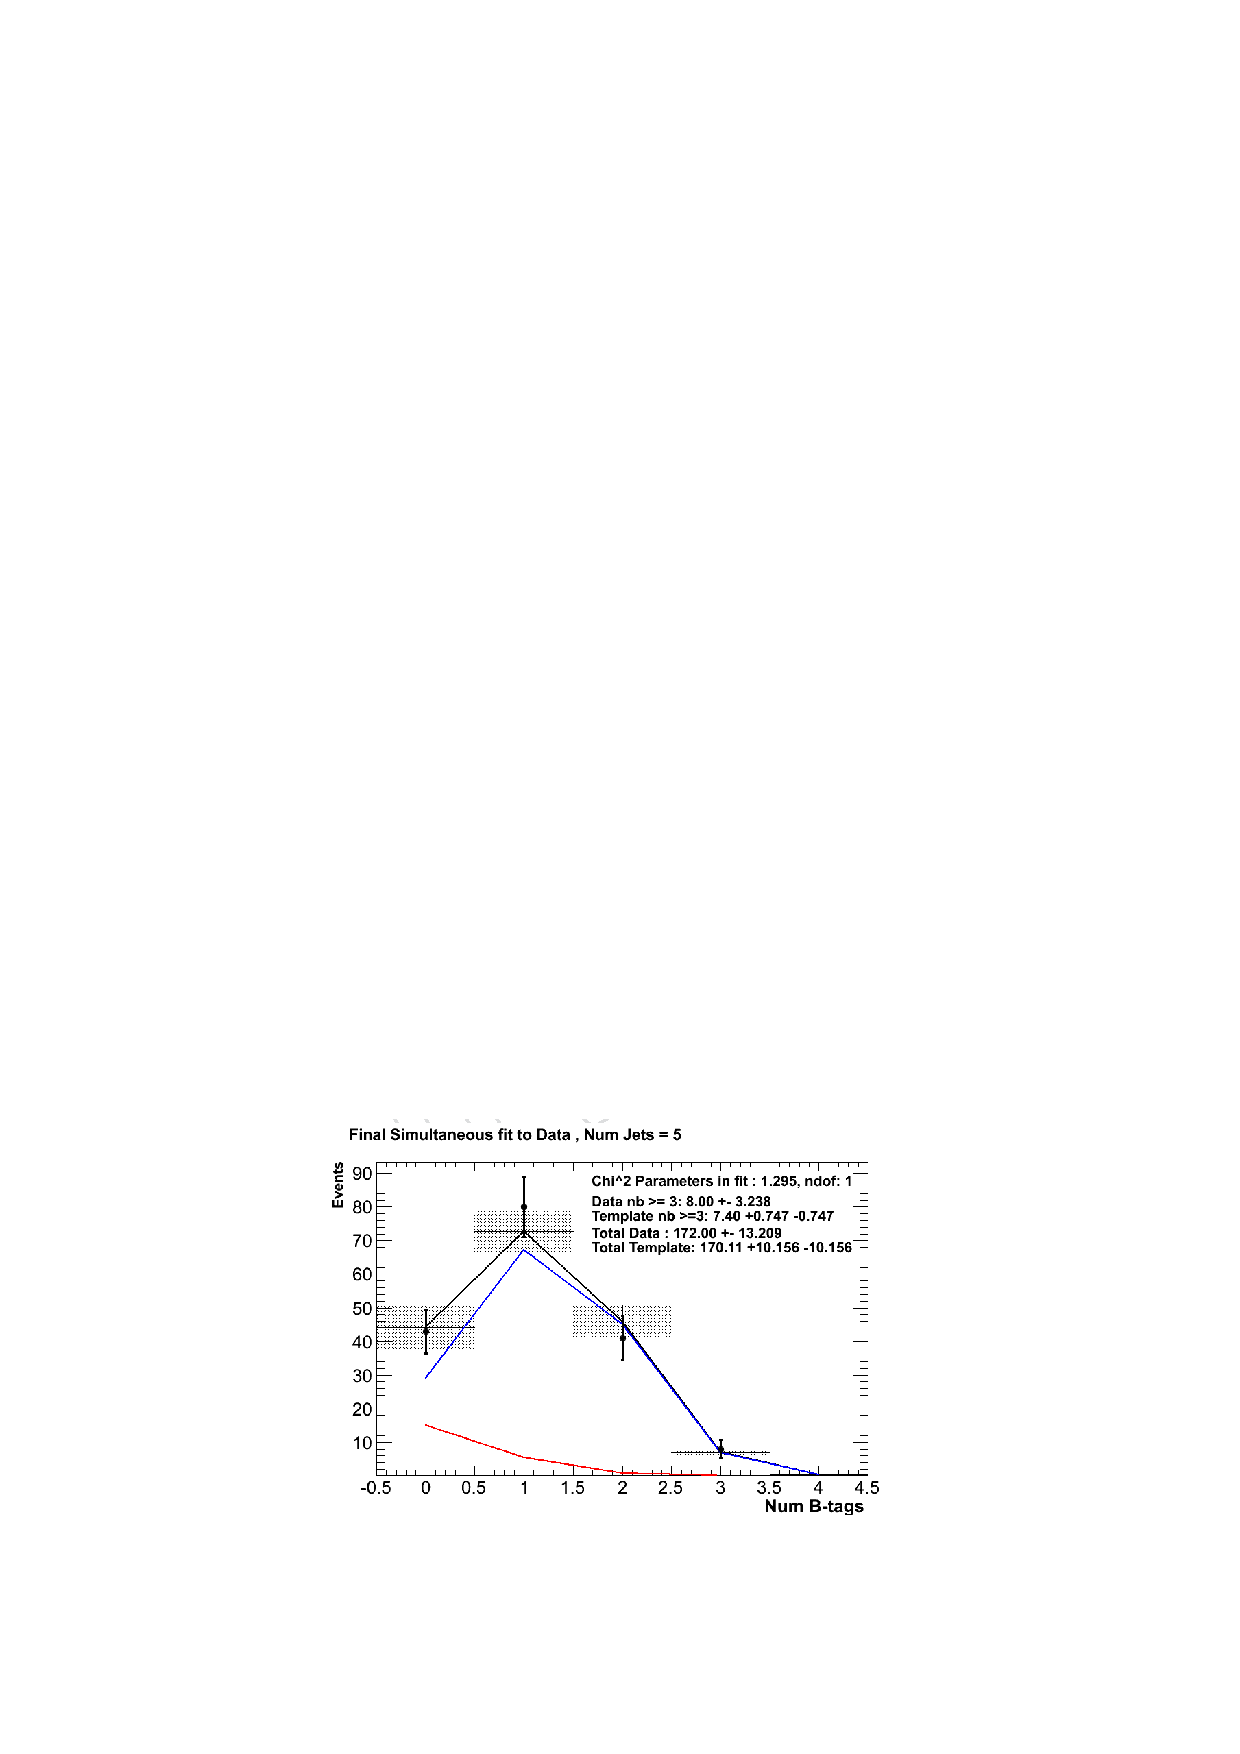
\includegraphics[width = 1.0\linewidth]{plots/template_data_medium_njet5_lowht.pdf}
\centering (a) $n_{jet} \geq$  5 , 275 $<$ \theht $<$ 325
\end{minipage}
\quad
\begin{minipage}[b]{0.55\linewidth}
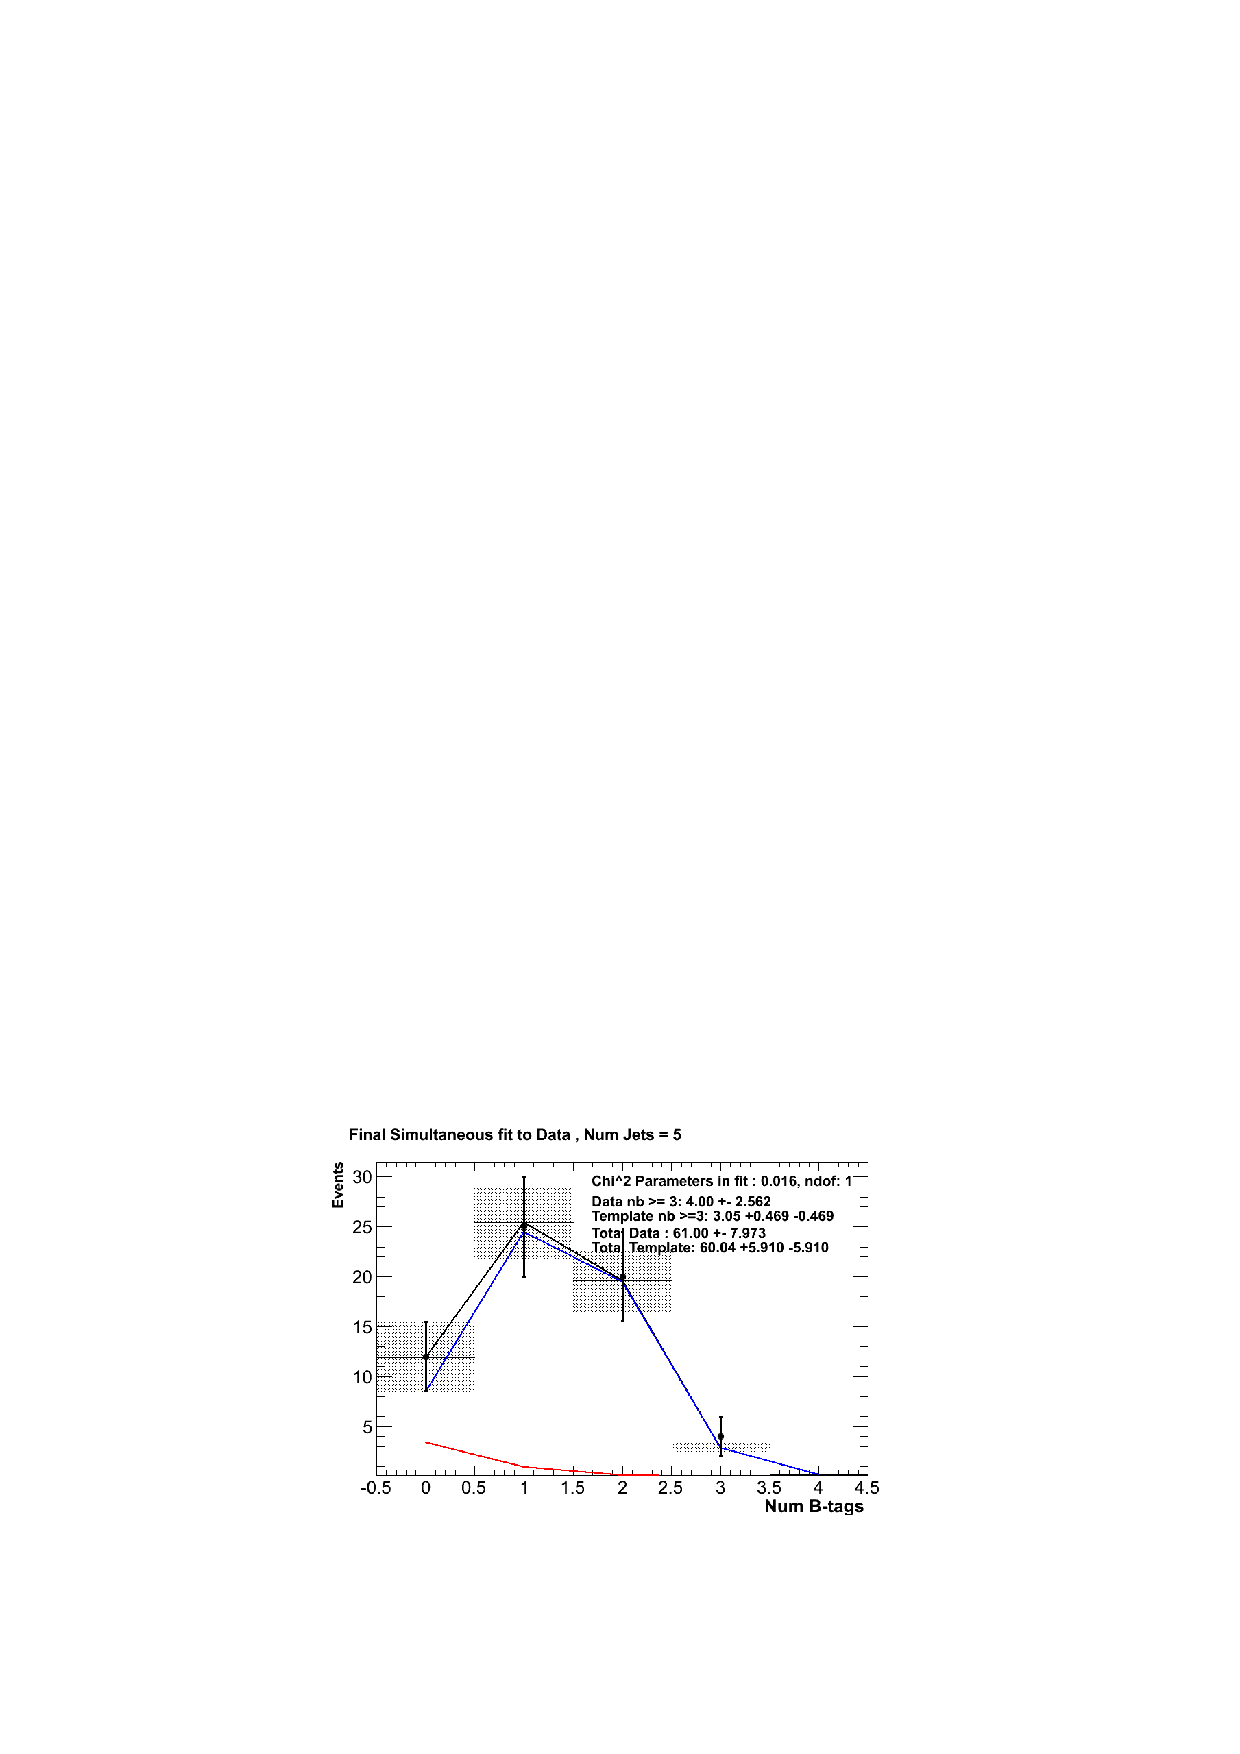
\includegraphics[width = 1.0\linewidth]{plots/template_data_medium_njet5_midht.pdf}
\centering (b) $n_{jet} \geq$ = 5 , 325 $<$ \theht $<$ 375 
\end{minipage}
\quad
\begin{minipage}[b]{0.55\linewidth}
\centering
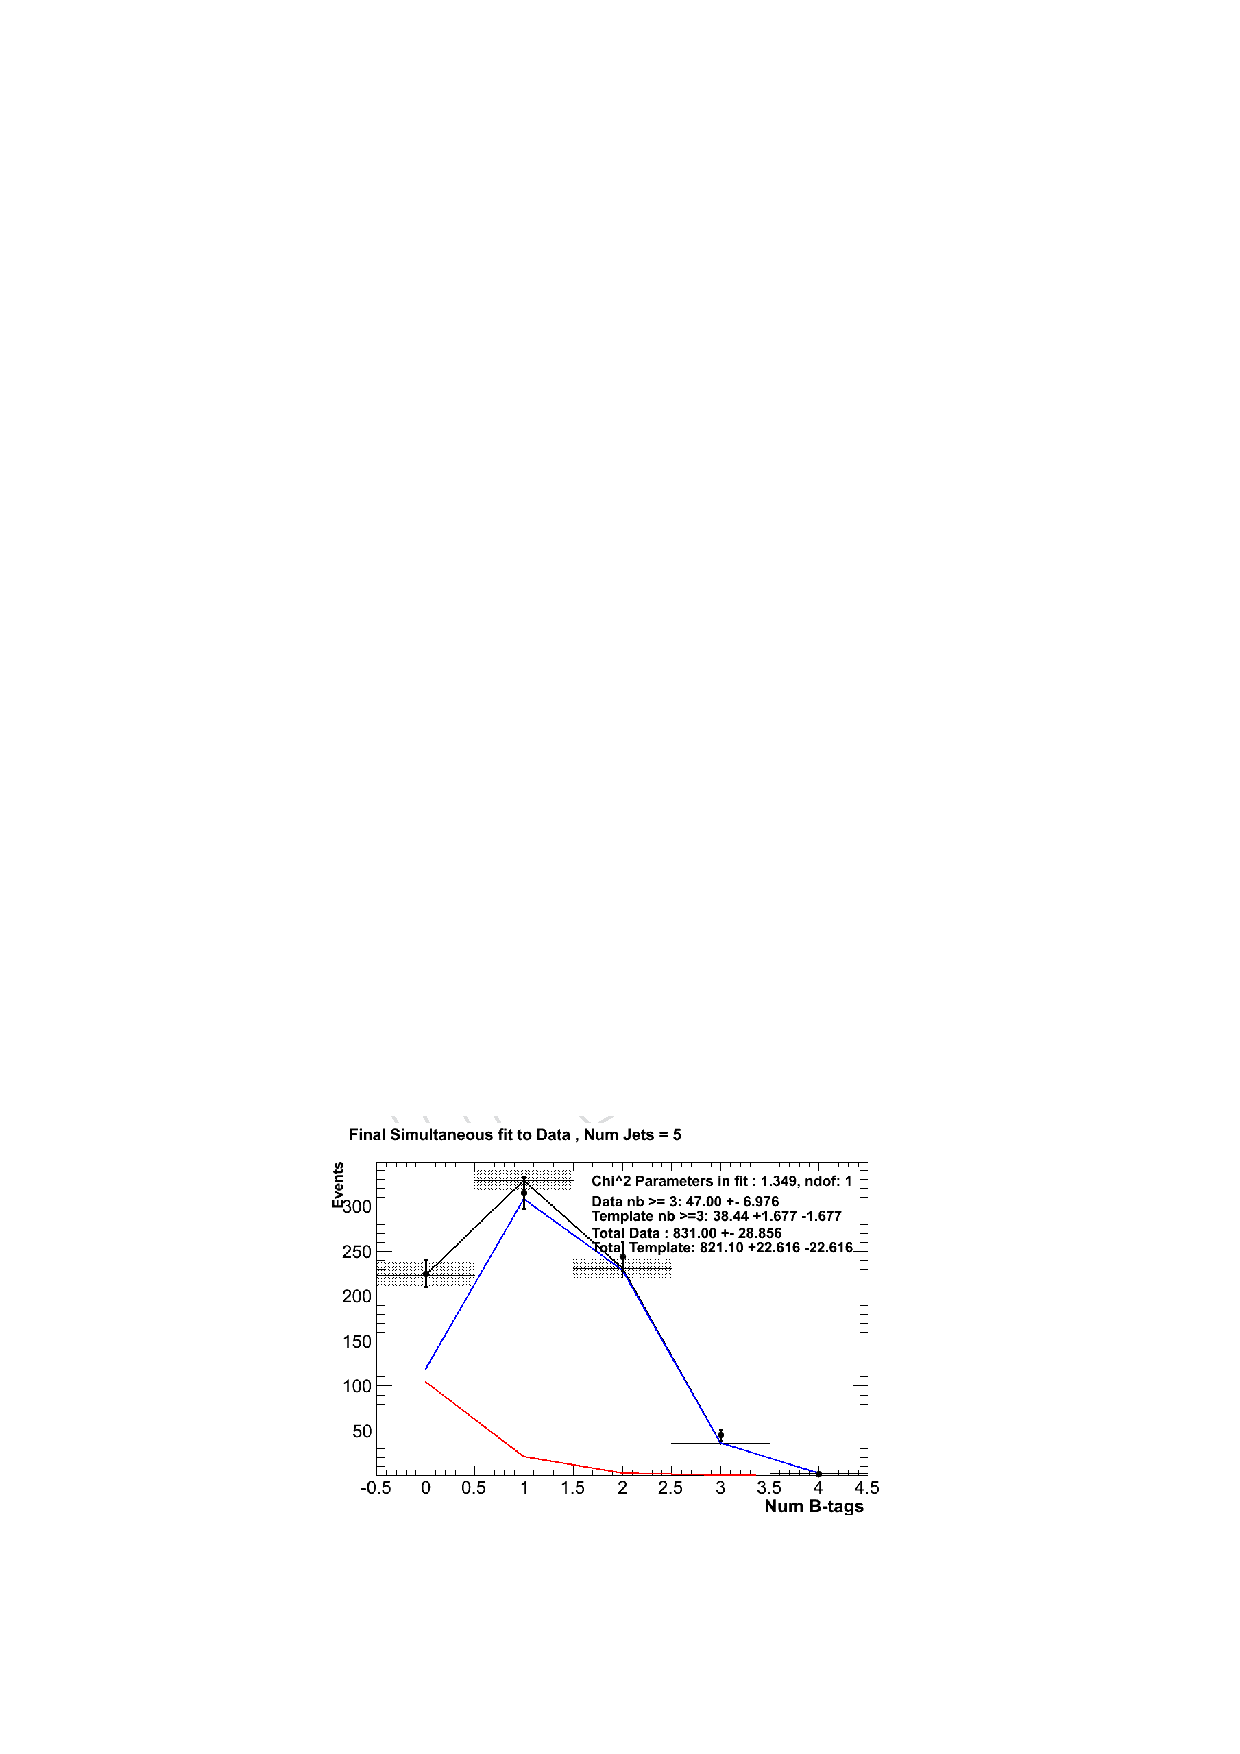
\includegraphics[width = 1.0\linewidth]{plots/template_data_medium_njet5_highht.pdf}
\centering (c) $n_{jet} \geq$ 5 , \theht $\geq$ 375 
\end{minipage}
\caption[The results of fitting the Z = 0 and Z = 2 templates to the $n_{b}^{reco}$ = 0, 1, 2 bins taken from data, for the $n_{jet} \geq 5$ category and medium \ac{CSV} working point.]{The results of fitting the Z = 0 and Z = 2 templates to the $n_{b}^{reco}$ = 0, 1, 2 bins taken directly from data, for the $n_{jet} \geq 5$ category and medium \ac{CSV} working point. The red template represents Z = 0, while the blue template represents Z = 2. The $\chi^{2}$ parameter displayed represents the goodness of fit to the low$ n_{b}^{reco}$ (0-2) control region.}
\label{fig:template_data_med_njet5}
\end{figure}

The numerical results and extrapolation to the $n_{b}^{reco} =$3,4 bins for all \theht and working points is shown in Table \ref{tab:template_datatable}.

 \begin{table}[h!]
\begin{center}
\footnotesize
\begin{tabular*}{0.95\textwidth}{@{\extracolsep{\fill}}llll}
\cline{1-4}
\multicolumn{1}{c}{\theht} & 275-325 & 325-375 & $>$375 \\
\multicolumn{4}{c}{Loose working point} \\
\hline\hline
Data $n_{b} = 3$ & 717 & 338 & 618\\ 
Template $n_{b} = 3$ & $782.6 \pm 16.8$ & $340.6 \pm 10.2$ & $601.9 \pm 14.2$ \\ 
Data $n_{b} = 4$ & 68 & 39 & 68 \\ 
Template $n_{b} = 4$ & $75.0 \pm 2.7$ & $27.6 \pm 1.3$ & $71.6 \pm 2.6$ \\ 
\hline
\multicolumn{4}{c}{Medium working point} \\
\hline\hline
Data $n_{b} = 3$ & 124 & 73 & 137 \\ 
Template $n_{b} = 3$ & $124.3 \pm 2.3$ & $62.0 \pm 1.7$ & $121.9 \pm 2.5$ \\ 
Data $n_{b} = 4$ & 1 & 1 & 3 \\ 
Template $n_{b} = 4$ & $2.6 \pm 0.1$ & $1.3 \pm 0.1$ & $4.0 \pm 0.1$ \\ 
\hline
\multicolumn{4}{c}{Tight working point} \\
\hline\hline
Data $n_{b} = 3$ & 21 & 13 & 23 \\ 
Template $n_{b} = 3$ & $26.7 \pm 0.5$ & $11.7 \pm 0.3$ & $21.9 \pm 0.5$ \\ 
Data $n_{b} = 4$ & 0 & 0 & 0 \\ 
Template $n_{b} = 4$ & $0.23 \pm 0.07$ & $0.09 \pm 0.04$ & $0.29 \pm 0.09$ \\ 
\end{tabular*}
\end{center}
\caption[Summary of the fit predictions in the $n_{b}^{reco}$ signal region of the \mupjets control sample, for $n_{jet} = 3, =4, \geq 5$. The fit region is $n_{b}^{reco}$ = 0, 1, 2 using 11.5 fb$^{-1}$ of data at $\sqrt{s} = 8$\TeV.]{Summary of the fit predictions in the $n_{b}^{reco}$ signal region of the \mupjets control sample, for $n_{jet} = 3, =4, \geq 5$. The fit region is $n_{b}^{reco}$ = 0, 1, 2 using 11.5 fb$^{-1}$ of data at $\sqrt{s} = 8$\TeV. The uncertainties quoted on the template yields are purely statistical.}\label{tab:template_datatable}
\end{table}

\FloatBarrier

The agreement for all working points demonstrates a good control of the b-tagging efficiency and mis-tagging rates and gives confidence in the method outlined. 

\subsection{Application to the \alphat hadronic search region}
\label{subsec:templatedataresults}

As an accompaniment to the background estimation methods outlined by the \alphat search. The b-tag template method offers a complimentary way of estimated the background within the hadronic signal region of the search�.


\section{Conclusions}
\label{subsec:templateconclusions}

A \ac{SUSY} signature such as one from gluino-induced third-generation squark production, would result in a final state with an underlying b-quark content greater than two. In order to be able to discriminate such signatures from the \ac{SM} background, templates are generated based on a parameterisation of the number of the \ac{SM} processes, where the underlying b-quarks per event is typically zero or two. These templates are then fit to data in a low $n_{b}^{reco}$ (0-2) control region in order to extrapolate a prediction in a high $n_{b}^{reco}$ (3-4) signal region. 

The method was demonstrated both in simulation and also in data, using the \ac{SM} enriched \mupjets selection from the \alphat search, to prove conceptually and experimentally that the method works and there is adequate control over the efficiency and mis-tagging rates in data for all working points of the \ac{CSV} tagger. Additionally this method was also applied to the \alphat analysis signal region where good agreement is observed between data and the background estimation method of the \alphat analysis.

